%%%%%%%%%%%%%%%%%%%%%%%%%%%%%%%%%%%%%%%%%%%%%%%%%%%%%%%%%%%%%%%%%%%%%%%%%%%%%%%%
\chapter{Literature Review}\label{ch:literature-review}
%%%%%%%%%%%%%%%%%%%%%%%%%%%%%%%%%%%%%%%%%%%%%%%%%%%%%%%%%%%%%%%%%%%%%%%%%%%%%%%%

%%%%%%%%%%%%%%%%%%%%%%%%%%%%%%%%%%%%%%%%%%%%%%%%%%%%%%%%%%%%%%%%%%%%%%%%%%%%%%%%
\section{Traffic Generators}\label{sec:traffic-gen}



Traffic generators are tools to transfer or inject network packets in a controlled manner,  aiming not at the actual data transfer data, but validation and performance benchmarking of devices under test (DUT)\cite{validate-trafficgen}. There is a vast variety of traffic generators described on literature \cite{ditg-paper} and available in the open-source community\footnote{\href{http://www.icir.org/models/trafficgenerators.html}{http://www.icir.org/models/trafficgenerators.html}}. 

Together with many traffic generators, there are many open-source APIs for traffic generation. Some are low-level APIs, which enables precise control of each packet generated, and are used in the implementation of traffic generators\footnote{For example: D-ITG\cite{ditg-paper} and Iperf\cite{web-iperf} uses the GNU Socket API\cite{web-socket}, Ostinato\cite{web-ostinato} uses libpcap\cite{web-libpcap}, and MoonGen\cite{moongen-paper} uses DPDK\cite{web-dpdk}. }. Also, they are computationally more efficient compared to high-level APIs for traffic generation. We've listed some low-level APIs below:

\begin{itemize}
\item GNU Socket API (C)\cite{web-socket};
\item Libpcap (C)\cite{web-libpcap};
\item Libtins (C++)\cite{web-libtins};
\item Scapy (Python)\cite{web-scrapy};
\item DPDK (C)\cite{web-dpdk}.
\end{itemize}

We also have high-level  APIs, usually provide by traffic generator, which simplifies the programming of custom traffic. For example:

\begin{itemize}
\item D-ITG API (C)\cite{web-ditg};
\item Ostinato API (Python)\cite{web-ostinato};
\item MoonGen API (Lua)\cite{web-moongen};
\item DPDK-Pktgen scripting interface (Lua)\cite{web-dpdk-pktgen}.
\end{itemize}

There are many taxonomies for traffic generators available on the literature. Classify traffic generators is usually "blur" process since packet generators feature many times fall in more than one class. We present two  taxonomies: 

\begin{itemize}
\item Traffic generation strategy;
\item Traffic generator implementation.
\end{itemize}

%%%%%%%%%%%%%%%%%%%%%%%%%%%%%%%%%%%%%%%%%%%%%%%%%%%%%%%%%%%%%%%%%%%%%%%%%%%%%%%
\subsection{Traffic generators by strategy}


Traffic generators can be classified into two main groups: replay engines\cite{sourcesonoff-paper} and model-based tools:

\begin{itemize}
\item \textbf{Replay engines}: These tools can read pcap files, and inject copies of the packet on a network interface. Eg.: TCPReplay\cite{web-tcpreplay}, TCPivo\cite{tcpivo-paper}, D-ITG\cite{ditg-paper}.
\item \textbf{Model-based traffic generators}: they generate synthetic traffic, controlling one or more feature of the traffic; such as header fields, packet sizes and inter-packet times.  
\end{itemize}

Model-based traffic generators can be sub-classified based on the abstraction layer the model operates. We follow here the taxonomy presented by Botta et al.\cite{do-you-trust}. Figure~\ref{fig:layers-workload-tools} shows these traffic generators organized in a layer diagram.

\begin{itemize}

\item \textbf{Application-level traffic generators}: they try to emulate the behavior of network applications, simulating real workloads stochastically or responsively 3. As an example, we have Surge, which emulates the communication between clients and web
servers;

\item \textbf{Flow-level traffic generators}: they can reproduce flow characteristics, such as flow duration, start times distributions, and temporal diurnal traffic volumes. Harpoon can extract these parameters from Cisco NetFlow data, collected from routers;

\item \textbf{Packet-level traffic generators}: it is the most used traffic generators. They can control packet-features like inter-departure times, packet size, throughput and packets per second. For example, D-ITG\cite{ditg-paper}, and TG\cite{web-tg} can control inter-packet times via stochastic distributions. However, most of them only permit the configuration of constant-rate models, by setting the packet rate or the traffic bandwidth, such as Iperf\cite{web-iperf}, BRUNO\cite{bruno-paper} and Ostinato\cite{web-ostinato}.

\item \textbf{Multi-level traffic generators}: this is a more recent class of network traffic generator. They take into account existing interaction among each layer of the network stack, to create network traffic as close as possible to reality. The most relevant tool is Swing\cite{swing-paper} which input collected pcap files. 

\end{itemize}


We have done an extensive survey on packet generators available on the open-source community, and classified them according to the first taxonomy. Also, we summarized the main features of each one. The result of this work is the tables \label{tab:app-level-tg}, \label{tab:multi-level-tg}, \label{tab:packet-level-tg}, and \label{tab:replay-tg}, in the appendix ~\ref{ap:traffic-gen-survey}. We also have a list of the tool repositories at table~\ref{tab:traffic-gen-links}


%%%%%%%%%%%%%%%%%%%%%%%%%%%%%%%%%%%%%%%%%%%%%%%%%%%%%%%%%%%%%%%%%%%%%%%%%%%%%%%
\subsection{According to the implementation of traffic generators}

\begin{itemize}

\item \textbf{Software-only traffic generators}: Implementations of traffic generators utterly independent of its running hardware platform. This implementation comprehends most of traffic generator tools, including all previously mentioned. 

\item \textbf{Software and hardware-dependent traffic generators}: are traffic generators implemented in software, but dependent on the underlying hardware. The most preeminent examples of this class used DPDK\cite{web-dpdk} as packet-generator API. DPDK works directly on the \acrshort{NIC} interface, avoiding overheads of the Operational System. As cited on its official website, this approach permits huge precision. As examples we have MoonGen\cite{moongen-paper} and DPDK-PktGen\cite{web-dpdk-pktgen}

\item \textbf{Hardware traffic generators}: these open-source traffic generators are implemented in hardware description language (VHDL/Verilog), and work on \acrshort{NetFPGA}s. Some examples of implementations are PacketGenerator\cite{pktgen-netfpga-paper}, Caliper\cite{caliper-paper}, and OSNT Packet Generator\cite{osnt-paper}.

\end{itemize}


\begin{figure}[!ht]
	\centering
	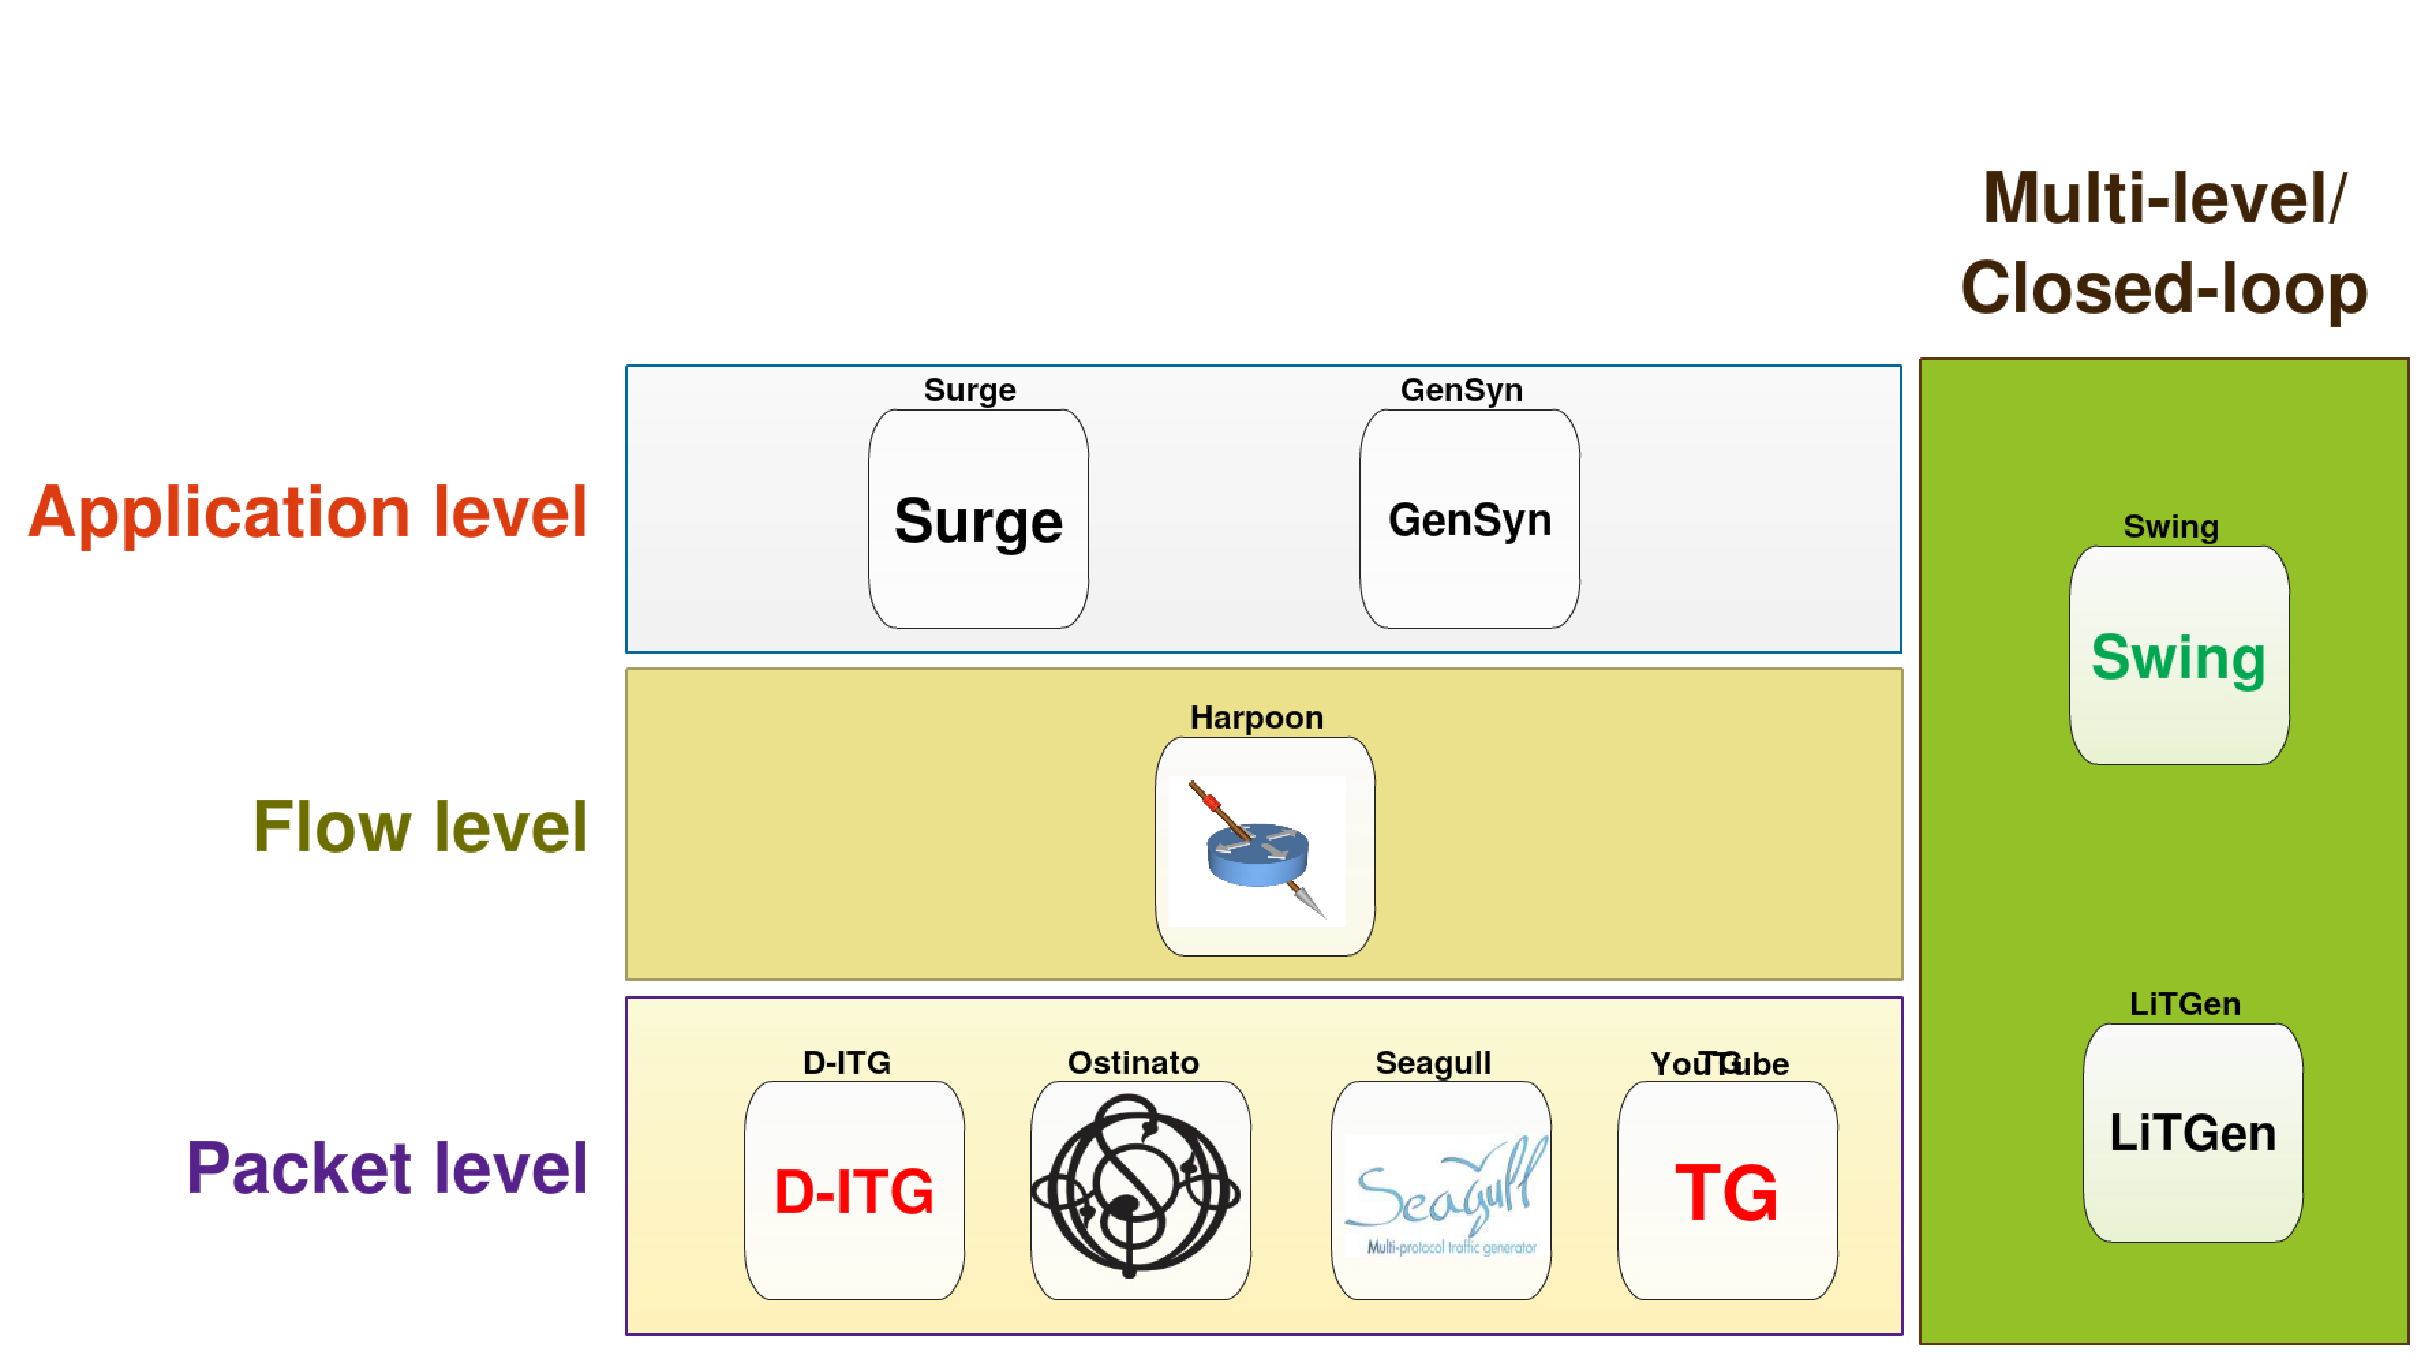
\includegraphics[scale=0.4]{figures/ch2/types-workload-tools}
	\caption{Diagram representing different traffic generators, according to its abstraction layer.}
	\label{fig:layers-workload-tools}
\end{figure}





%%%%%%%%%%%%%%%%%%%%%%%%%%%%%%%%%%%%%%%%%%%%%%%%%%%%%%%%%%%%%%%%%%%%%%%%%%%%%%%
\section{Realistic Traffic and Traffic Modeling}\label{sec:modeling-traffic}

\subsection{Realistic Network Traffic Generation}

As presented, there is a considerable amount of open-source traffic generators available, each one of them with many different sets of features available. However, on the generation of realistic workload, the set of possibilities become much more restricted. On the other hand, there are many works on characterization, modeling, and simulation of different types of network workload. As stated by Botta et al., a synthetic network traffic generation over real networks should be able to: 

\begin{enumerate}
\item Capture real traces complexity over different scenarios;
\item Be able to custom change some specific properties of the generated traffic ;
\item Return measure indicators of performance experienced by the workload.
\end{enumerate}


As we have found out over the literature in our research, the measure of realism of a traffic generator is given by how well a traffic generator can represent features at the level its model works. For example:

\begin{itemize}
\item \textbf{Swing}: Vishwanath and Vahdat\cite{swing-paper} validate their work against packet, flow, and application level features;
\item \textbf{Harpoon}: Sommers and Barford\cite{harpoon-validation} validate harpoon on flow-level features;
\item \textbf{D-ITG}: Botta et al.\cite{ditg-paper} validate their work against application-level and packet-level features;
\item \textbf{sourcesOnOff}: Varet and Larrieu validate sourcesOnOff on packet-level features\cite{sourcesonoff-paper}. 
\end{itemize}

Therefore, we defined a realistic traffic generator as follows:

\vspace{5mm}
\begin{tcolorbox}[colback=blue!5,colframe=blue!40!black,title=Realistic Traffic Generator]
A realistic traffic generator is a tool that its model can reproduce real traces complexity and behavior, at the same level of abstraction its traffic model works: on the packet, flow, application or multi-level. In other words, the validation techniques must give similar results to the real and synthetic traces. 
\end{tcolorbox}
\vspace{5mm}

We are going to discuss metrics on validation of traffic generators in the next section. The rest of this section will highlight topics on network traffic modeling. We are not going to discuss application modeling, since each one may have their specific behavior. We are going to discuss points that apply to any traffic in general:

\begin{itemize}
\item Inter-packet times (throughput) modeling;
\item Packet-sizes modeling;
\item Packet-header fields;
\item Flow modeling;
\item Closed-loop behavior modeling.
\end{itemize}

%%%%%%%%%%%%%%%%%%%%%%%%%%%%%%%%%%%%%%%%%%%%%%%%%%%%%%%%%%%%%%%%%%%%%%%%%%%%%%%
\subsection{Inter-packet times (throughput) modeling}


\begin{table}[t!]
\centering
\caption{Probability density function (\acrshort{PDF}) and Cumulative distribution function (\acrshort{CDF}) of some random variables, and if this stochastic distribution has or not self-similarity property. Some functions used to express these distributions are defined at the table ~\ref{tab:distributions-definitions} }
\label{tab:distributions-equations}
\scalebox{0.82}{ 
\begin{tabular}{lcccr}
Distribution & PDF Equation & CDF Equation & Parameters & Heavy-tailed\\ \hline
\\
\multirow{2}{*}{Poisson} & \multirow{2}{*}{$f[k] = \frac{e^{-\lambda}\lambda^k}{k!}$} & \multirow{2}{*}{$F[k] = \frac{\Gamma(\lfloor k + 1 \rfloor, \lambda)}{ \lfloor k \rfloor!}$} &  $\lambda > 0$  (mean, \\
 &  &  & variance) & no \\ 
\\ 
\multirow{2}{*}{Binomial} & \multirow{2}{*}{$f[k] = \binom{n}{k}p^{k}(1 - p)^{n - k} $} & \multirow{2}{*}{$F[k] = I_{1 - p}(n - k, 1 + k)$} &  $n > 0$ (trials)\\  &  &  &$p > 0$ (success)  & no \\ 
\\
\multirow{2}{*}{Normal} & \multirow{2}{*}{$f(t) =  \frac{1}{\sqrt[]{2\sigma^2}\pi}e^{\frac{(t - \mu)^2}{2\sigma^2}}$ } & \multirow{2}{*}{ $F(t) = \frac{1}{2}[ 1 + \text{erf}(\frac{t - \mu}{\sigma\sqrt[]{2}})]$ } &  $\mu$ (mean) \\ &  &  & $\sigma > 0$ (std.dev) & no \\ 
\\ 
\multirow{2}{*}{Exponential} & \multirow{2}{*}{ $f(t) = \begin{cases} \lambda e^{-\lambda t} ;& t \geq 0 \\ 0;& t < 0 \end{cases} $  }   & \multirow{2}{*}{ $F(t) = 1 - e^{-\lambda t} $ } & \\ &  &  & $\lambda > 0$ (rate)  & no \\ 
\\
\multirow{2}{*}{Pareto} & \multirow{2}{*}{$f(t) = \begin{cases} \frac{\alpha t_{m}^\alpha}{t^{\alpha + 1}} ;& t \geq t_{m} \\ 0;& t < t_{m} \end{cases} $ } & \multirow{2}{*}{$F(t) = \begin{cases} 1 - (\frac{t_{m}}{t})^\alpha ;& t \geq t_{m} \\ 0;& t < t_{m}\end{cases} $} &  $\alpha > 0$ (shape)  \\ & &  &  $t_{m} > 0$ (scale)   & yes \\ 
\\ 
\multirow{2}{*}{Cauchy} & \multirow{2}{*}{ $f(t) = \frac{1}{\pi \gamma}[\frac{\gamma^2}{(t - t_{0})^{2} + \gamma^{2}}]$ } & \multirow{2}{*}{ $F(t) = \frac{1}{\pi}\arctan( \frac{t - t_{0}}{\gamma} ) + \frac{1}{2}  $ } &  $\gamma > 0$ (scale) \\ &  &   & $t_{0} > 0$ (location) & yes \\  
\\
\multirow{2}{*}{Weibull} & \multirow{2}{*}{ $f(t) = \begin{cases} \frac{\alpha}{\beta^\alpha}t^{\alpha - 1}e^{(t/\beta)^{\alpha}}; & t \geq 0 \\ 0; & t < 0 \end{cases}$  } & \multirow{2}{*}{ $F(t) = \begin{cases} 1 - e^{-(t/\beta)^{\alpha}}; & t \geq 0 \\ 0 ; & t < 0  \end{cases}$ } & $\alpha  > 0 $ (shape) \\ &  &  & $\beta > 0$ (scale)  & yes \\
\\
\multirow{2}{*}{Gamma} & \multirow{2}{*}{ $ f(t) = \frac{\beta^{\alpha}}{\Gamma(\alpha)}t^{\alpha - 1}e^{-\beta t}  $ } & \multirow{2}{*}{$ F(t) = 1 - \frac{1}{\Gamma(\alpha)}\Gamma(\alpha, \beta x) $} & $\alpha > 0$ (shape) \\ &  &  & $\beta > 0$ (rate) & no \\
\\ 
%\multirow{2}{*}{Student's t} & \multirow{2}{*}{} & \multirow{2}{*}{} &  \\ &  &  & & \\ 
%\\
\multirow{2}{*}{Beta} & \multirow{2}{*}{ $ f(t) = \frac{x^{\alpha - 1}(1 - x)^{\beta - 1}}{B(\alpha, \beta)} $ } & \multirow{2}{*}{ $ F(t) = I_{x}(\alpha, \beta) $ } &  $\alpha > 0$ (shape) \\ &  &  & $\beta > 0$ (shape) & no \\ 
\\ 
\multirow{2}{*}{Log-normal} & \multirow{2}{*}{ $ f(t) = \frac{1}{t \sigma \sqrt[]{2 \pi}}e^{- \frac{(\ln(x) - \mu)^{2}}{2 \sigma^{2}}} $ } & \multirow{2}{*}{ $ F(t) = \frac{1}{2} + \frac{1}{2}\text{erf}[\frac{\ln(x) - \mu}{\sqrt[]{2} \sigma}] $ } & $\mu$ (location)\\
 &  &  & $ \sigma > 0 $ (shape) & yes \\ 
\\
\multirow{2}{*}{Chi-squared} & \multirow{2}{*}{ $ f(t) = \frac{1}{2^{\frac{k}{2}}\Gamma(\frac{k}{2}) }t^{\frac{k}{2} - 1}e^{-\frac{t}{2}} $ } & \multirow{2}{*}{ $ F(t) = \frac{1}{\Gamma(\frac{k}{2})}\gamma(\frac{k}{2}, \frac{x}{2}) $ } &  \\
 &  &  & $ k \in \mathbb{N}_{>0} $ &  no\\ 
\\
 
\hline
\end{tabular} 
} %scalebox
\end{table}

\begin{table}[t!]
\centering
\caption{Definitions of some functions used by PDFs and CDFs}
\label{tab:distributions-definitions}
\begin{tabular}{ll}
\hline
Function                             & Definition \\ 
\hline
\\
Regularized Incomplete beta function & $ I_{x}(a, b) = \frac{B(x| a, b)}{B(a, b)} $           \\
\\
Incomplete beta function             & $ B(x| a, b) = \int_{0}^{x} t^{a - 1} (1 - t)^{(b - 1)} \text{d}t $           \\
\\
Beta function                        & $ B(x| a, b) = \int_{0}^{1} t^{a - 1} (1 - t)^{(b - 1)} \text{d}t $           \\
\\
Error function                       & $ \text{erf}(x) = \frac{1}{\sqrt[]{\pi}}\int_{x}^{-x} e^{-t^{2}} \text{d}t $           \\ 
\\
Lower incomplete Gamma function      & $ \gamma(s, x) = x^{s}\Gamma(s)e^{-x}\sum_{k = 0}^{\infty}\frac{x^{k}}{\Gamma(s+k+1)} $  \\
\\
\hline
\end{tabular}
\end{table}


Classical models for network traffic generation were the same used in telephone traffic, such as  Poisson or Poisson-related, like Markov and Poisson-batch. They can describe the randomness of an Ethernet link but cannot capture the presence of "burstiness" in a long-term time scale, such as traffic "spikes" on long-range "ripples". Lerand et al.\cite{selfsimilar-ethernet}, points in his seminal work, in 1994, that the nature of the Ethernet traffic is self-similar. It has a fractal-like shape since characteristics seen in a small time scale should appear on a long-scale as well, that have been referred, in the most of the time, as long-range dependence or degree of long-range dependence (LRD). One way to identify if a process is self-similar is by checking its Hurst parameter, or Hurst exponent H, as a measure of the "burstiness" and LRD.  A random process is self-similar and LRD if $0.5 < H <1$\cite{stochastic-selfsimilar}. 

Willinger et al. pointed out that the Ethernet traffic has a high variability (or infinite variance)\cite{selfsimilar-highvariability}.  Processes with such characteristic are said to be heavy-tailed. In practical terms, that means a sudden discontinuous change can always occur. Heavy tail shows that a stochastic distribution is not exponentially bounded. In other words, some value far from the mean does not have a negligible probability of occurrence. We can express self-similar and heavy-tailed processes using heavy-tailed stochastic distributions, such as Pareto and Weibull. Table~\ref{tab:distributions-equations} shows the reference for these stochastic distributions. In the last column, we indicate if the distribution is or not heavy-tailed. 

These concepts of  High variability and Self-similarity are called Noah and Joseph Effects\cite{selfsimilar-highvariability}. Willinger et al. point that the superposition of many ON/OFF sources (or packet trains) using ON and OFF times that obey the Noah Effect (heavy-tailed probabilistic functions), also obey the Joseph effect. That means, it is a self-similar process and can be used to describe Ethernet traffic. Some works on the literature on synthetic traffic uses this principle, like sourcesOnOff\cite{sourcesonoff-paper}, or have to heavy-tailed processes, such as like D-ITG.

Furthermore, some later studies advocate the use of more advanced multiscaling models (multifractal), addressed by investigations that uses envelope processes\cite{envelope-process}. 


%%%%%%%%%%%%%%%%%%%%%%%%%%%%%%%%%%%%%%%%%%%%%%%%%%%%%%%%%%%%%%%%%%%%%%%%%%%%%%%
\subsection{Packet-sizes modeling}


\begin{table}[t!]
\centering
\caption{Two different studies evaluating the impact of packet size on the throughput. Both compare many available open-source tools on different testbeds. In all cases, small packet sizes penalize the throughput. Bigger packet sizes achieve a higher throughput.}
\label{tab:packet-size-impact}
\scalebox{0.9}{
\begin{tabular}{|l|c|c|c|}
\hline
 & \multicolumn{3}{c|}{Traffic Generators} \\ \cline{2-4} 
\multicolumn{1}{|c|}{Article and setup} &  & \multicolumn{1}{c|}{Maximum bit-rate} & \multicolumn{1}{c|}{Maximum bit-rate} \\
 & \multicolumn{1}{c|}{Toll} & \multicolumn{1}{c|}{\begin{tabular}[c]{@{}c@{}}at small packet \\ sizes\end{tabular}} & \multicolumn{1}{c|}{\begin{tabular}[c]{@{}c@{}}at big packet \\ sizes\end{tabular}} \\ \hline
\textit{\begin{tabular}[c]{@{}l@{}}Comparative study of various \\ Traffic Generator Tools \cite{comparative-trafficgen-tools} ;\end{tabular}} & PackETH & 150 @(64 bytes) & 1745 @(1408 bytes) \\ \cline{2-4} 
\begin{tabular}[c]{@{}l@{}}setup: Linux (Centos 6.2, \\ Kernel version 2.6.32),\end{tabular} & Ostinato & 135 @(64 bytes) & 2850 @(1408 bytes) \\ \cline{2-4} 
\begin{tabular}[c]{@{}l@{}}Inter(R) Xeon(R) CPU with 2.96GHz,\\  RAM of 64GB , NIC Mellanox\end{tabular} & D-ITG & 62 @(64 bytes) & 1950 @(1408 bytes), \\
\begin{tabular}[c]{@{}l@{}}Technologies MT25418 {[}ConnectXVPI \\ PCIe 2.0 2.5GT/s - IB DDR{]}\end{tabular} &  &  & \begin{tabular}[c]{@{}l@{}}9808 @(1460 bytes, \\ 12 threads)\end{tabular} \\ \cline{2-4} 
10 Bbps. Protocol: TCP & Iperf & * & \begin{tabular}[c]{@{}l@{}}8450 @(1460 bytes, \\ 12 threads)\end{tabular} \\ \hline
\textit{\begin{tabular}[c]{@{}l@{}}Performance Monitoring of Various \\ Network Traffic Generators \cite{performance-trafficgen};\end{tabular}} & Iperf & 46.0 @(128 bytes) & 93.1 @(1408 bytes) \\ \cline{2-4} 
\begin{tabular}[c]{@{}l@{}}Inter(R) Pentium 4(R), CPU \\ with 3.0GHz, RAM 1GB,\end{tabular} & Netperf & 46.0 @(128 bytes) & 89.9 @(1408 bytes) \\ \cline{2-4} 
\begin{tabular}[c]{@{}l@{}}NIC Intel Pro/100 Adapter \\ (100Mbps),\end{tabular} & D-ITG & 38.1 @(128 bytes) & 83.1 @(1408 bytes) \\ \cline{2-4} 
\begin{tabular}[c]{@{}l@{}}Hard Drivers Seagate Barracuda \\ 7200 series with 20BG. \\ Protocol:TCP\end{tabular} & IP Traffic & 61.0 @(128 bytes) & 76.7 @(1408 bytes) \\ \hline
\end{tabular}
}
\end{table}

The literature shows that the packet size of a trace may result in a considerable impact in a trace throughput since small packets cause a significant overhead on packet processing\cite{stochastic-selfsimilar}\cite{performance-trafficgen}. Table~\ref{tab:packet-size-impact} summarizes the results from two different works about throughput impact of packet sizes. On packet size distributions’ characterization, we can find many works as well.  For example, Castro et al. pointed that  90\% of \acrshort{UDP} packets were smaller than 500 bytes, and most packets transmitted using \acrshort{TCP} have 40 bytes (acknowledgment) and 1500 bytes (Maximum Transmission Unit, MTU)\cite{packet-distribution-model}. Ostrowsky et al.  found that on UDP traces, the modes of two regions were 120 and 1350 bytes, with a cut-off value of 750 bytes. They also found that roughly UDP packets constituted 20\% of the total number of packets on captures\cite{udp-flows-model}. Castro et al. points on his work that capture traces made on routers were all bimodal, and the majority is TCP. However, the size of each mode may change depending on the application. For example, an \acrshort{HTTP} traffic tends to have a mode closer to the \acrshort{MTU} compared to an \acrshort{FTP} capture\cite{packet-distribution-model}.


%%%%%%%%%%%%%%%%%%%%%%%%%%%%%%%%%%%%%%%%%%%%%%%%%%%%%%%%%%%%%%%%%%%%%%%%%%%%%%%
\subsection{Packet-header fields}

Accurate replication of network traffic should be able to control packet headers such as protocols, ports, addresses, and so on. Traffic generators provide support for these features, more frequently in a limited way. Most offer support just common protocols, such as TCP, UDP, and \acrshort{IPv4}. On the other hands, there are some which provide a vast variety of support and control over packet headers like PackETH\cite{web-packeth} and D-ITG\cite{web-ditg}. Other tools are even able to enable someone to extend this feature and develop support to new protocols. For example, Ostinato and Seagull permit the customization and creation of protocols\cite{wp-seagull}.


%%%%%%%%%%%%%%%%%%%%%%%%%%%%%%%%%%%%%%%%%%%%%%%%%%%%%%%%%%%%%%%%%%%%%%%%%%%%%%%
\subsection{Flow modeling}

Some packet-level traffic generators permit the control of flow generation, mostly manually through an API or scripting. In terms of automatic flow configuration, an example is Harpoon\cite{harpoon-paper}, which can to automatically configure its flows, using as input NetFlow Cisco traffic traces to automatically setting parameters. Harpoon deals with flow modeling in three different levels: file level, session level, and user level, not dealing with packet level at all. In the file level, Harpoon model two parameters: the files size and the time interval between consecutive file requests, called inter-file request time. The middle level is the session level, that consist of sequences files transfer between two distinct \acrshort{IP} addresses. The session level has three components: the IP spatial distribution, the second is the inter-session start times and the third is the session duration. The last level is the user level. In Harpoon, "users" are divided on "TCP" and "UDP" users, which conduct consecutive session using these protocols. This level has two components: the user ON time, and the number of active users. By modeling the number of users, Harpoon can reproduce temporal (diurnal) traffic volumes.


%%%%%%%%%%%%%%%%%%%%%%%%%%%%%%%%%%%%%%%%%%%%%%%%%%%%%%%%%%%%%%%%%%%%%%%%%%%%%%%
\subsection{Closed-loop(responsive) models}

The closed-loop operation means that the traffic generator uses feedback to reconfigure its model. That means the traffic generator can change its behavior at run time according to the observation made in real-time, changing the traffic created. These modifications involve changes on parameters of statistical distributions of inter-departure time and packet size, for example. Swing\cite{swing-paper} and application-level traffic generators like Surge\cite{surge-paper} and GenSyn\cite{gensyn-paper}uses this strategy.





%%%%%%%%%%%%%%%%%%%%%%%%%%%%%%%%%%%%%%%%%%%%%%%%%%%%%%%%%%%%%%%%%%%%%%%%%%%%%%%%
\section{Validation of Traffic Generator Tools}~\label{sec:validation-traffic-gen}


After the implementation of a traffic generator, it needs to be validated. Thus, we need a set of proof of concepts to evaluate if it reached its purposes or not. Researchers have been proposed many validation techniques, according to the traffic generator intended behavior. Magyesi and Szabó\cite{validate-trafficgen} presented a survey of these techniques, grouped by type of metric. The authors classified the techniques into four categories: packet based metrics, flow-based metrics, scaling characteristics, and \acrshort{QoS}/\acrshort{QoE} related metrics. Here we present a short review of each group of these validation techniques.


%%%%%%%%%%%%%%%%%%%%%%%%%%%%%%%%%%%%%%%%%%%%%%%%%%%%%%%%%%%%%%%%%%%%%%%%%%%%%%%%
\subsection{Packet Based Metrics}

Packet-based metrics are the most used metrics in the validation of traffic generators\cite{validate-trafficgen}. The most relevant packet based metrics are throughput\cite{do-you-trust}\cite{comparative-trafficgen-tools}\cite{performance-trafficgen}\cite{moongen-paper} (bytes and packets), packet size distribution\cite{packet-distribution-model} and inter-packet time distribution (inter-arrival and inter-departure)\cite{sourcesonoff-paper} \cite{ditg-paper}.


%%%%%%%%%%%%%%%%%%%%%%%%%%%%%%%%%%%%%%%%%%%%%%%%%%%%%%%%%%%%%%%%%%%%%%%%%%%%%%%%
\subsection{Flow Based Metrics}


Flow-based metrics are becoming more critical since newer network elements, like SDN devices, can execute flow-based operations\cite{validate-trafficgen}\cite{sdn-survey}. Magyesi and Szabó\cite{validate-trafficgen} consider the essential flow metrics, the flow size distribution, and volume. The flow volume stands for the number of flows of traffic. The flow size distribution is a measure of the length on time from the flows in network traffic. The flow volume is proportional to the number of flow instances that a flow-based device should run simultaneously. Moreover, the flow sizes define how much time each of these instances will run.


%%%%%%%%%%%%%%%%%%%%%%%%%%%%%%%%%%%%%%%%%%%%%%%%%%%%%%%%%%%%%%%%%%%%%%%%%%%%%%%%
\subsection{Fractal and Scaling Characteristics}

Second order characteristics such as "burstiness" and long-range dependence are responsible for the complex nature of internet traffic\cite{validate-trafficgen}. Due to its non-stationary nature, traditional methods fail to extract useful information\cite{validate-trafficgen}. The first analysis made in that way focused on the estimation of the Hurst exponent\cite{selfsimilar-ethernet}. They demonstrated the self-similar nature of the Ethernet traffic. As explained before, self-similar traffic should be in a Hurst exponent $H$, such as $0.5 < H < 1$. Over the years, wavelet-based analysis has become an efficient way to reveal correlations, bursts and scaling nature of the Ethernet traffic\cite{validate-trafficgen}. Many papers have used wavelet-based analysiscite{swing-paper}\cite{non-intrusive-wavelet}\cite{wavelet-analysis-long-range}. Huang et al.\cite{non-intrusive-wavelet} and Abry and Veitch\cite{wavelet-analysis-long-range} offer an extensible explanation of wavelet-based scaling analysis (\acrshort{WSA}) or wavelet multi-resolution energy analysis (\acrshort{WMA}). The explanation about the primary information offered by these two works will be showed below. 

First, consider a time series $X_{0,k}$ for $k = 0, 1, ... 2^n$:

\begin{equation}
\{X_{0,k}\} = \{ X_{0,0}, X_{0,1}, ... ,X_{0,2^{n}} \}
\end{equation} 

Suppose that we coarser $X_{0}$ in another time-series $X_{1}$ with half of the original resolution, but using  $ \sqrt[]{2} $ as normalization factor:

\begin{equation}
X_{1,k} = \frac{1}{\sqrt{2}}(X_{0,2k} + X_{0,2k+1})
\end{equation}

If we take the differences, instead of the averages, evaluate the so-called \textit{details}.

\begin{equation}
d_{1,k} = \frac{1}{\sqrt{2}}(X_{0,2k} - X_{0,2k+1})
\end{equation}

We can continue repeating this process, writing more coarse time series $X_{2}$ from $X_{1}$, until we reach $X_{n}$. Therefore, we will get a collection of \textit{details}:

\begin{equation}
\{d_{j,k}\} = \{ d_{1,0}, d_{1,1}, ..., d_{1,2^{n/2}}, ..., d_{n, 0} \}
\end{equation}

This collection of details ${d_{j,k}}$ are called Discrete Haar Wavelet Transform. Using the \textit{details}, we can calculate the energy function $E_{j}$, for each scale $j$, using:

\begin{equation}
E_{j} = \frac{1}{N_{j}} \sum_{k = 0}^{N_{j} - 1} |d_{j,k}|^{2}; \qquad j = 1, 2, ..., n
\end{equation} 
\\ 
were $N_{j}$ is the total number of coefficients at scale $j$. If we plot $\log(E_{j})$ as a function o the scale $j$, we will obtain a wavelet multiresolution energy plot.

On energy wavelet multiresolution energy plots, it is possible to capture three different central behavior, according to the scale. On \textbf{periodic time series}, the Energy values will be small. In fact, on perfectly periodic scales $j$, the values of the energy function $E_{j}$ will be zero. So periodicity will be sensed if the value of the energy function decrease. Perfect \textbf{white noise time series} will maintain the same value of the energy function. So an approximately constant value for the energy function $E_{j}$ indicates white noise behavior (which can be represented by a Poisson process\cite{poisson-white-noise}). On \textbf{self-similar time series}, the energy function plot $\log(E_{j})$ grows approximately linearly with the scale $j$. This characteristic explains why it has become a standard for realistic traffic generation analysis. In a single plot, we can quickly identify periodicities, and self-similar and Poisson process characteristics, just seeing if it decays, grow, or remain constant.

Later studies suggested the use of multi-fractal models, instead of the self-similar models (also called monofractal)\cite{validate-trafficgen}\cite{udp-flows-model}. Since there is a lack of multiscaling analysis on validation of traffic generation in the literature, this type of analysis will stay for future works.

\begin{figure*}[ht!]
	\centering
	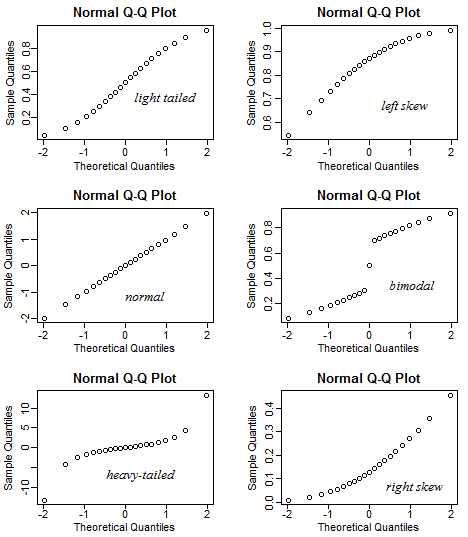
\includegraphics[width=0.6\textwidth]{figures/ch2/qqplot-tutorial}
	\caption{ How information about may be extracted from QQplots.}
	\label{fig:qqplot-tutorial}
\end{figure*}


Another way to analyze scaling characteristics is through QQplots. \acrshort{QQplot} is a visual method to compare sample data with a specific stochastic distribution. It orders the sample data values from the smallest to largest, then plots these values against the expected value given by the probability distribution function. The data sample values appear along the y-axis and the expected values along the x-axis. The more linear, the more the data is likely to be expressed by this specific stochastic distribution. 

Depending on how the plot behaves, some features of the empirical dataset compared to the theoretical can be observed. Figure~\ref{fig:qqplot-tutorial} presents a summary.


%%%%%%%%%%%%%%%%%%%%%%%%%%%%%%%%%%%%%%%%%%%%%%%%%%%%%%%%%%%%%%%%%%%%%%%%%%%%%%%%
\subsection{QoS/QoE Related Metrics}


For the point of view of traffic generation, QoS and QoE metrics should present similar values to the ones found in real scenarios. As stated by Magyesi and Szabó\cite{validate-trafficgen}, important QoS/QoE metrics on validation of workload tools are Round trip Time values (\acrshort{RTT}), average queue waiting time and, queue size. Still, on queue size, self-similar traffic consumes router buffers faster than Poisson traffic\cite{multi-player-online-game-self-similarity}.

%%%%%%%%%%%%%%%%%%%%%%%%%%%%%%%%%%%%%%%%%%%%%%%%%%%%%%%%%%%%%%%%%%%%%%%%%%%%%%%%
\section{Conclusions}


In this chapter, we discussed some fundamental concepts of our research: network traffic generators, network traffic modeling, and network traffic generators validation. In section~\ref{sec:traffic-gen}, we surveyed types of traffic generators and a comparison between their considerable variability of features. It helped us to summarize and have an understanding of what is available nowadays for use, and define the gaps. Also, this chapter helped us to identify what tools and frameworks are available to use. Section~\ref{sec:modeling-traffic} showed a brief overview of efforts on network traffic modeling and realistic traffic generation. In the modeling issue, was presented a short historical summary of some critical points of network traffic modeling, and on practical traffic generation, discussing some reference tools.


